\documentclass[journal,12pt,two column]{IEEEtran}
%\usepackage{setspace}
\usepackage{amssymb}
\usepackage[cmex10]{amsmath}
\usepackage{amsthm}
\usepackage[export]{adjustbox}
\usepackage{bm}
\def\inputGnumericTable{} 
\usepackage[latin1]{inputenc}                                 
\usepackage{color}                                            
\usepackage{array} 
\usepackage{longtable} 
\usepackage{calc}                                             
\usepackage{multirow}                                         
\usepackage{hhline}                                           
\usepackage{ifthen}  
\usepackage{mathtools}
\usepackage{tikz}
\usepackage{listings}
\usepackage{color}                                            %%
\usepackage{array}                                            %%
\usepackage{caption} 
\usepackage{graphicx}
\usepackage[latin1]{inputenc}                                 
\usepackage{color}                                            
\usepackage{array}                                            
\usepackage{longtable}                                        
\usepackage{calc}                                             
\usepackage{multirow}                                         
\usepackage{hhline}                                           
\usepackage{ifthen}  

\renewcommand\thesection{\arabic{section}}
\renewcommand\thesubsection{\thesection.\arabic{subsection}}
\renewcommand\thesubsubsection{\thesubsection.\arabic{subsubsection}}

\renewcommand\thesectiondis{\arabic{section}}
\renewcommand\thesubsectiondis{\thesectiondis.\arabic{subsection}}
\renewcommand\thesubsubsectiondis{\thesubsectiondis.\arabic{subsubsection}}
\title{Assignment}
\author{Barath surya M \\ EE22BTECH11014}

% correct bad hyphenation here
\hyphenation{op-tical net-works semi-conduc-tor}
\def\inputGnumericTable{}                                 %%

\lstset{
%language=C,
frame=single, 
breaklines=true,
columns=fullflexible
}
%\lstset{
%language=tex,
%frame=single, 
%breaklines=true
%}


\providecommand{\pr}[1]{\ensuremath{\Pr\left(#1\right)}}
\providecommand{\prt}[2]{\ensuremath{p_{#1}^{\left(#2\right)} }}        % own macro for this question
\providecommand{\qfunc}[1]{\ensuremath{Q\left(#1\right)}}
\providecommand{\sbrak}[1]{\ensuremath{{}\left[#1\right]}}
\providecommand{\lsbrak}[1]{\ensuremath{{}\left[#1\right.}}
\providecommand{\rsbrak}[1]{\ensuremath{{}\left.#1\right]}}
\providecommand{\brak}[1]{\ensuremath{\left(#1\right)}}
\providecommand{\lbrak}[1]{\ensuremath{\left(#1\right.}}
\providecommand{\rbrak}[1]{\ensuremath{\left.#1\right)}}
\providecommand{\cbrak}[1]{\ensuremath{\left\{#1\right\}}}
\providecommand{\lcbrak}[1]{\ensuremath{\left\{#1\right.}}
\providecommand{\rcbrak}[1]{\ensuremath{\left.#1\right\}}}
\newcommand{\sgn}{\mathop{\mathrm{sgn}}}
\providecommand{\abs}[1]{\left\vert#1\right\vert}
\providecommand{\res}[1]{\Res\displaylimits_{#1}} 
\providecommand{\norm}[1]{\left\lVert#1\right\rVert}
%\providecommand{\norm}[1]{\lVert#1\rVert}
\providecommand{\mtx}[1]{\mathbf{#1}}
\providecommand{\mean}[1]{E\left[ #1 \right]}
\providecommand{\cond}[2]{#1\middle|#2}
\providecommand{\fourier}{\overset{\mathcal{F}}{ \rightleftharpoons}}
%\providecommand{\hilbert}{\overset{\mathcal{H}}{ \rightleftharpoons}}
%\providecommand{\system}{\overset{\mathcal{H}}{ \longleftrightarrow}}
 %\newcommand{\solution}[2]{\textbf{Solution:}{#1}}
\newcommand{\solution}{\noindent \textbf{Solution: }}
\newcommand{\cosec}{\,\text{cosec}\,}
\providecommand{\dec}[2]{\ensuremath{\overset{#1}{\underset{#2}{\gtrless}}}}
\newcommand{\myvec}[1]{\ensuremath{\begin{pmatrix}#1\end{pmatrix}}}
\newcommand{\mydet}[1]{\ensuremath{\begin{vmatrix}#1\end{vmatrix}}}
\providecommand{\rank}{\text{rank}}
\providecommand{\pr}[1]{\ensuremath{\Pr\left(#1\right)}}
\providecommand{\qfunc}[1]{\ensuremath{Q\left(#1\right)}}
 \newcommand*{\permcomb}[4][0mu]{{{}^{#3}\mkern#1#2_{#4}}}
\newcommand*{\perm}[1][-3mu]{\permcomb[#1]{P}}
\newcommand*{\comb}[1][-1mu]{\permcomb[#1]{C}}
\providecommand{\qfunc}[1]{\ensuremath{Q\left(#1\right)}}
\providecommand{\gauss}[2]{\mathcal{N}\ensuremath{\left(#1,#2\right)}}
\providecommand{\diff}[2]{\ensuremath{\frac{d{#1}}{d{#2}}}}
\providecommand{\myceil}[1]{\left \lceil #1 \right \rceil }
\newcommand\figref{Fig.~\ref}
\newcommand\tabref{Table~\ref}
\newcommand{\sinc}{\,\text{sinc}\,}
\newcommand{\rect}{\,\text{rect}\,}
%%
% %\newcommand{\solution}[2]{\textbf{Solution:}{#1}}
%\newcommand{\solution}{\noindent \textbf{Solution:

%\newcommand{\cosec}{\,\text{cosec}\,}
%\numberwithin{equation}{section}
%\numberwithin{equation}{subsection}
%\numberwithin{problem}{section}
%\numberwithin{definition}{section}
%\makeatletter
%\@addtoreset{figure}{problem}
%\makeatother

%\let\StandardTheFigure\thefigure
\let\vec\mathbf

\begin{document}
\maketitle
Consider the experiment of throwing a die. If a multiple of 3 comes up, throw the die again. If any other number comes up, toss a coin. Find the conditional probability of the event the coin shows a tail, given that  at least one die shows a 3.\\
\solution
\begin{table}[ht!]
	%%%%%%%%%%%%%%%%%%%%%%%%%%%%%%%%%%%%%%%%%%%%%%%%%%%%%%%%%%%%%%%%%%%%%%
%%                                                                  %%
%%  This is the header of a LaTeX2e file exported from Gnumeric.    %%
%%                                                                  %%
%%  This file can be compiled as it stands or included in another   %%
%%  LaTeX document. The table is based on the longtable package so  %%
%%  the longtable options (headers, footers...) can be set in the   %%
%%  preamble section below (see PRAMBLE).                           %%
%%                                                                  %%
%%  To include the file in another, the following two lines must be %%
%%  in the including file:                                          %%
%%        \def\inputGnumericTable{}                                 %%
%%  at the beginning of the file and:                               %%
%%        \input{name-of-this-file.tex}                             %%
%%  where the table is to be placed. Note also that the including   %%
%%  file must use the following packages for the table to be        %%
%%  rendered correctly:                                             %%
%%    \usepackage[latin1]{inputenc}                                 %%
%%    \usepackage{color}                                            %%
%%    \usepackage{array}                                            %%
%%    \usepackage{longtable}                                        %%
%%    \usepackage{calc}                                             %%
%%    \usepackage{multirow}                                         %%
%%    \usepackage{hhline}                                           %%
%%    \usepackage{ifthen}                                           %%
%%  optionally (for landscape tables embedded in another document): %%
%%    \usepackage{lscape}                                           %%
%%                                                                  %%
%%%%%%%%%%%%%%%%%%%%%%%%%%%%%%%%%%%%%%%%%%%%%%%%%%%%%%%%%%%%%%%%%%%%%%



%%  This section checks if we are begin input into another file or  %%
%%  the file will be compiled alone. First use a macro taken from   %%
%%  the TeXbook ex 7.7 (suggestion of Han-Wen Nienhuys).            %%
\def\ifundefined#1{\expandafter\ifx\csname#1\endcsname\relax}


%%  Check for the \def token for inputed files. If it is not        %%
%%  defined, the file will be processed as a standalone and the     %%
%%  preamble will be used.                                          %%
\ifundefined{inputGnumericTable}

%%  We must be able to close or not the document at the end.        %%
	\def\gnumericTableEnd{\end{document}}


%%%%%%%%%%%%%%%%%%%%%%%%%%%%%%%%%%%%%%%%%%%%%%%%%%%%%%%%%%%%%%%%%%%%%%
%%                                                                  %%
%%  This is the PREAMBLE. Change these values to get the right      %%
%%  paper size and other niceties.                                  %%
%%                                                                  %%
%%%%%%%%%%%%%%%%%%%%%%%%%%%%%%%%%%%%%%%%%%%%%%%%%%%%%%%%%%%%%%%%%%%%%%

	\documentclass[12pt%
			  %,landscape%
                    ]{report}
       \usepackage[latin1]{inputenc}
       \usepackage{fullpage}
       \usepackage{color}
       \usepackage{array}
       \usepackage{longtable}
       \usepackage{calc}
       \usepackage{multirow}
       \usepackage{hhline}
       \usepackage{ifthen}

	\begin{document}


%%  End of the preamble for the standalone. The next section is for %%
%%  documents which are included into other LaTeX2e files.          %%
\else

%%  We are not a stand alone document. For a regular table, we will %%
%%  have no preamble and only define the closing to mean nothing.   %%
    \def\gnumericTableEnd{}

%%  If we want landscape mode in an embedded document, comment out  %%
%%  the line above and uncomment the two below. The table will      %%
%%  begin on a new page and run in landscape mode.                  %%
%       \def\gnumericTableEnd{\end{landscape}}
%       \begin{landscape}


%%  End of the else clause for this file being \input.              %%
\fi

%%%%%%%%%%%%%%%%%%%%%%%%%%%%%%%%%%%%%%%%%%%%%%%%%%%%%%%%%%%%%%%%%%%%%%
%%                                                                  %%
%%  The rest is the gnumeric table, except for the closing          %%
%%  statement. Changes below will alter the table's appearance.     %%
%%                                                                  %%
%%%%%%%%%%%%%%%%%%%%%%%%%%%%%%%%%%%%%%%%%%%%%%%%%%%%%%%%%%%%%%%%%%%%%%

\providecommand{\gnumericmathit}[1]{#1} 
%%  Uncomment the next line if you would like your numbers to be in %%
%%  italics if they are italizised in the gnumeric table.           %%
%\renewcommand{\gnumericmathit}[1]{\mathit{#1}}
\providecommand{\gnumericPB}[1]%
{\let\gnumericTemp=\\#1\let\\=\gnumericTemp\hspace{0pt}}
 \ifundefined{gnumericTableWidthDefined}
        \newlength{\gnumericTableWidth}
        \newlength{\gnumericTableWidthComplete}
        \newlength{\gnumericMultiRowLength}
        \global\def\gnumericTableWidthDefined{}
 \fi
%% The following setting protects this code from babel shorthands.  %%
 \ifthenelse{\isundefined{\languageshorthands}}{}{\languageshorthands{english}}
%%  The default table format retains the relative column widths of  %%
%%  gnumeric. They can easily be changed to c, r or l. In that case %%
%%  you may want to comment out the next line and uncomment the one %%
%%  thereafter                                                      %%
\providecommand\gnumbox{\makebox[0pt]}
%%\providecommand\gnumbox[1][]{\makebox}

%% to adjust positions in multirow situations                       %%
\setlength{\bigstrutjot}{\jot}
\setlength{\extrarowheight}{\doublerulesep}

%%  The \setlongtables command keeps column widths the same across  %%
%%  pages. Simply comment out next line for varying column widths.  %%
\setlongtables

\setlength\gnumericTableWidth{%
	250pt+%
	139pt+%
	442pt+%
0pt}
\def\gumericNumCols{3}
\setlength\gnumericTableWidthComplete{\gnumericTableWidth+%
         \tabcolsep*\gumericNumCols*2+\arrayrulewidth*\gumericNumCols}
\ifthenelse{\lengthtest{\gnumericTableWidthComplete > \linewidth}}%
         {\def\gnumericScale{1*\ratio{\linewidth-%
                        \tabcolsep*\gumericNumCols*2-%
                        \arrayrulewidth*\gumericNumCols}%
{\gnumericTableWidth}}}%
{\def\gnumericScale{1}}

%%%%%%%%%%%%%%%%%%%%%%%%%%%%%%%%%%%%%%%%%%%%%%%%%%%%%%%%%%%%%%%%%%%%%%
%%                                                                  %%
%% The following are the widths of the various columns. We are      %%
%% defining them here because then they are easier to change.       %%
%% Depending on the cell formats we may use them more than once.    %%
%%                                                                  %%
%%%%%%%%%%%%%%%%%%%%%%%%%%%%%%%%%%%%%%%%%%%%%%%%%%%%%%%%%%%%%%%%%%%%%%

\ifthenelse{\isundefined{\gnumericColA}}{\newlength{\gnumericColA}}{}\settowidth{\gnumericColA}{\begin{tabular}{@{}p{250pt*\gnumericScale}@{}}x\end{tabular}}
\ifthenelse{\isundefined{\gnumericColB}}{\newlength{\gnumericColB}}{}\settowidth{\gnumericColB}{\begin{tabular}{@{}p{139pt*\gnumericScale}@{}}x\end{tabular}}
\ifthenelse{\isundefined{\gnumericColC}}{\newlength{\gnumericColC}}{}\settowidth{\gnumericColC}{\begin{tabular}{@{}p{442pt*\gnumericScale}@{}}x\end{tabular}}

\begin{tabular}[c]{%
	b{\gnumericColA}%
	b{\gnumericColB}%
	b{\gnumericColC}%
	}

%%%%%%%%%%%%%%%%%%%%%%%%%%%%%%%%%%%%%%%%%%%%%%%%%%%%%%%%%%%%%%%%%%%%%%
%%  The longtable options. (Caption, headers... see Goosens, p.124) %%
%	\caption{The Table Caption.}             \\	%
% \hline	% Across the top of the table.
%%  The rest of these options are table rows which are placed on    %%
%%  the first, last or every page. Use \multicolumn if you want.    %%

%%  Header for the first page.                                      %%
%	\multicolumn{3}{c}{The First Header} \\ \hline 
%	\multicolumn{1}{c}{colTag}	%Column 1
%	&\multicolumn{1}{c}{colTag}	%Column 2
%	&\multicolumn{1}{c}{colTag}	\\ \hline %Last column
%	\endfirsthead

%%  The running header definition.                                  %%
%	\hline
%	\multicolumn{3}{l}{\ldots\small\slshape continued} \\ \hline
%	\multicolumn{1}{c}{colTag}	%Column 1
%	&\multicolumn{1}{c}{colTag}	%Column 2
%	&\multicolumn{1}{c}{colTag}	\\ \hline %Last column
%	\endhead

%%  The running footer definition.                                  %%
%	\hline
%	\multicolumn{3}{r}{\small\slshape continued\ldots} \\
%	\endfoot

%%  The ending footer definition.                                   %%
%	\multicolumn{3}{c}{That's all folks} \\ \hline 
%	\endlastfoot
%%%%%%%%%%%%%%%%%%%%%%%%%%%%%%%%%%%%%%%%%%%%%%%%%%%%%%%%%%%%%%%%%%%%%%

\hhline{|-|-|-}
	 \multicolumn{1}{|p{\gnumericColA}|}%
	{\gnumericPB{\centering}\gnumbox{Random variable}}
	&\multicolumn{1}{p{\gnumericColB}|}%
	{\gnumericPB{\centering}\gnumbox{values}}
	&\multicolumn{1}{p{\gnumericColC}|}%
	{\gnumericPB{\centering}\gnumbox{Events}}
\\
\hhline{|---|}
	 \multicolumn{1}{|p{\gnumericColA}|}%
	{\setlength{\gnumericMultiRowLength}{0pt}%
	 \addtolength{\gnumericMultiRowLength}{\gnumericColA}%
	 \multirow{2}[1]{\gnumericMultiRowLength}{\parbox{\gnumericMultiRowLength}{%
	 \gnumericPB{\centering}\gnumbox{X}}}}
	&\multicolumn{1}{p{\gnumericColB}|}%
	{\gnumericPB{\centering}\gnumbox{0}}
	&\multicolumn{1}{p{\gnumericColC}|}%
	{\gnumericPB{\centering}\gnumbox{The numbers are consecutive}}
\\
\hhline{~|--|}
	 \multicolumn{1}{|p{\gnumericColA}|}%
	{}
	&\multicolumn{1}{p{\gnumericColB}|}%
	{\gnumericPB{\centering}\gnumbox{1}}
	&\multicolumn{1}{p{\gnumericColC}|}%
	{\gnumericPB{\centering}\gnumbox{The numbers are not consecutive}}
\\
\hhline{|-|-|-|}
\end{tabular}

\ifthenelse{\isundefined{\languageshorthands}}{}{\languageshorthands{\languagename}}
\gnumericTableEnd

\end{table}
Let, the states $S_0$ and $S_1$ describe the outcomes of dice throws.\\
$S_2$ and $S_3$ describe the outcomes of coin toss.
Conditional Probability is that "The coin shows tails" given that "at least one die shows a 3".
Since, a Markov chain does not depend on the past outcomes,
\begin{align}
    p_{S_3 | S_0}&=\pr{X_n=S_3|X_1 =S_0}
\end{align}
Transition Probability Matrix is given as,
\begin{align}
    \vec{P}&=\myvec{\frac{1}{3}&0&0&0\\
                    \frac{2}{3}&0&0&0\\
                    0&\frac{1}{2}&1&0\\
                    0&\frac{1}{2}&0&1
                }
\end{align}
The state vector is defined as,
\begin{align}
	\vec{Q_n}=\myvec{p_{S_0}^n\\p_{S_1}^n\\p_{S_2}^n\\p_{S_3}^n}
\end{align}
where $p_{S_i}^n$ is the probability of $S_i$ state after n time interval from initial state.\\
The given conditon is "3 occurs at least once", and we let occurrence of 3 as the initial state, Since Markov chain does not depend on past outcomes. So, $\pr{X=S_0}=1$ and 0 for all other states.\\
And State vector is ,
\begin{align}
    \vec{Q_0}=\myvec{1\\0\\0\\0}
\end{align}
the state vector after one step in time can be written as,
\begin{align}
    \vec{Q_1}&=\vec{P Q_0}\\
    \vec{Q_2}&=\vec{P Q_1}\\
    \vdots\\
    \vec{Q_{n}}&=\vec{P Q_{n-1}}
\end{align}
we can see that the markov chain is reducible, a unique state vector exists and it is equal to limiting distribution.i.e, after a long time,
\begin{align}
	\vec{Q_n}=\vec{Q_{n-1}}
\end{align}
substituting the chain of state vectors, we get
\begin{align}
    \vec{Q_{n}}&=\vec{P^n Q_0}
\end{align}
applying limits to find the stationary probability vector,
\begin{align}
     \lim_{n \to \infty} \vec{Q_{n}}&=\vec{Q}=\vec{P^n Q_0}
\end{align} \label{eq:steady}
We can find $Q$ using eigenvector and eigenvalues.
Now, to find the eigenvalues, let $\lambda$ be the eigen value for the Transition Probability matrix.
\begin{align}
	\implies |\vec{P} -\lambda \vec{I}|&=0\\
	\myvec{\frac{1}{3} -\lambda&0&0&0\\
                    \frac{2}{3}&0 - \lambda&0&0\\
                    0&\frac{1}{2}&1- \lambda&0\\
                    0&\frac{1}{2}&0&1-\lambda
                }&=0\\
                \brak{\frac{1}{3}-\lambda}\brak{1-\lambda}^2 \brak{-\lambda}&=0\\
                \implies \lambda&=\frac{1}{3},0,1,1
\end{align} 
Now, to find eigenvector,
\begin{align}
	|\vec{P}-\lambda \vec{I}|\vec{X}=0
\end{align}
where $X$ is the eigen vector coresponding to eigen value $\lambda$ , using row reduction\\
$\implies \lambda =\frac{1}{3}$
\begin{align}
	\vec{X}&=\myvec{\frac{-2}{3}\\\frac{-4}{3}\\1\\1}
\end{align}
$\implies \lambda =0$
\begin{align}
	\vec{X}&=\myvec{0\\-2\\1\\1}
\end{align}
$\implies \lambda = 1$
\begin{align}
	\vec{X}&=\myvec{0\\0\\1\\0}
\end{align}
also
\begin{align}
	\vec{X}&=\myvec{0\\0\\0\\1}
\end{align}
then the eigenvector matrix is ,
\begin{align}
	\vec{S}&=\myvec{\frac{-2}{3}&0&0&0\\
	\frac{-4}{3}&-2&0&0\\
	1&1&1&0\\
	1&1&0&1}
\end{align}
Diagonal matrix $\vec{D}$ is,
\begin{align}
	\vec{D}=\myvec{\frac{1}{3}&0&0&0\\
	0&0&0&0\\
	0&0&1&0\\
	0&0&0&1}
\end{align} 
It is said that,
\begin{align}
	\vec{P}&=\vec{S}\vec{D}\vec{S}^{-1}\\
	\implies \vec{P}^n&=\vec{S}\vec{D}^n \vec{S}^{-1}\\
	\implies \lim_{n \to \infty} \vec{P}^n&=\vec{S} \vec{D}^n \vec{S}^{-1}\\
\end{align}
finding as $n \to \infty$ , value of $\vec{D}$
\begin{align}
	\lim_{n \to \infty} \vec{D}^n&=\myvec{\brak{\frac{1}{3}}^n &0&0&0\\
	0&0&0&0\\
	0&0&1^n&0\\
	0&0&0&1^n}\\
	&=\myvec{0&0&0&0\\
	0&0&0&0\\
	0&0&1&0\\
	0&0&0&1}
\end{align}
\begin{align}	
	\lim _{n \to \infty}\vec{P}^n&=\vec{S}\vec{D}^n \vec{S}^{-1}\\
	&=\myvec{0&0&0&0\\0&0&0&0\\\frac{1}{2}&\frac{1}{2}&1&0\\ \frac{1}{2}&\frac{1}{2} &0&1}
\end{align}
By substituting the values of $Q_0$ and $P_\infty$ in the above equation, We get the steady state probability vector as,
\begin{align}
    \vec{Q}&=\myvec{0&0&0&0\\0&0&0&0\\\frac{1}{2}&\frac{1}{2}&1&0\\\frac{1}{2}&\frac{1}{2}&0&1}\myvec{1\\0\\0\\0}\\
    &=\myvec{0\\0\\\frac{1}{2}\\\frac{1}{2}}
\end{align}
So, the probability that "coin shows tails" given that "Die shows at least one 3" is,
\begin{align}
    p_{3|1} &= \frac{1}{2}
\end{align}
\begin{figure}[ht!]
    \centering
    \resizebox{.9\linewidth}{!}{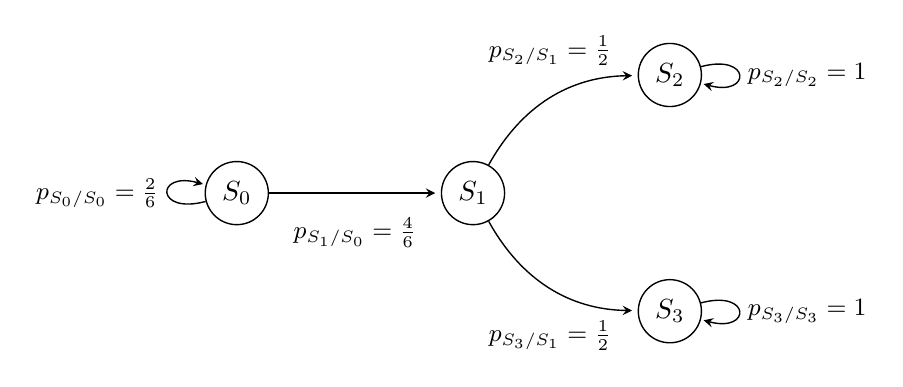
\begin{tikzpicture}[->, >= stealth, shorten >=2pt, line width=0.5pt, node distance=2cm]
  \node[circle, draw] (A) at (0, 1.5) {$S_0$};
  \node[circle, draw] (B) at (3, 1.5) {$S_1$};
  \node[circle, draw] (C) at (5.5, 3) {$S_2$};
  \node[circle, draw] (D) at (5.5, 0) {$S_3$};
  
  \begin{small}
    \path (A) edge [loop left] node [left] {$p_{S_0/S_0} = \frac{2}{6}$} (A);
    \path (A) edge node [below = 0.2cm] {$p_{S_1/S_0} = \frac{4}{6}$} (B);
  
    \path (B) edge [bend left] node [above = 0.3cm] {$p_{S_2/S_1} = \frac{1}{2}$} (C);
    \path (B) edge [bend right] node [below = 0.3cm] {$p_{S_3/S_1} = \frac{1}{2}$} (D);
  
    \path (C) edge [loop right] node {$p_{S_2/S_2} = 1$} (C);
    \path (D) edge [loop right] node {$p_{S_3/S_3} = 1$} (D);
  \end{small}
\end{tikzpicture}
}
    \caption{State diagram generated using LatexTikZ}
    \label{fig:Statediagramdiecoin}
\end{figure}
\end{document}
